\section{Esquematização do conteúdo das páginas}

Para ser possibilitar a perceção dos dados necessários para alimentar o \textit{software}, o que apresentar em cada página e também como navegar entre os ecrãs da aplicação foi então desenhado um esquema 
(Figura~\ref{fig:3}).

\begin{figure}[htb]
    \centering
    
    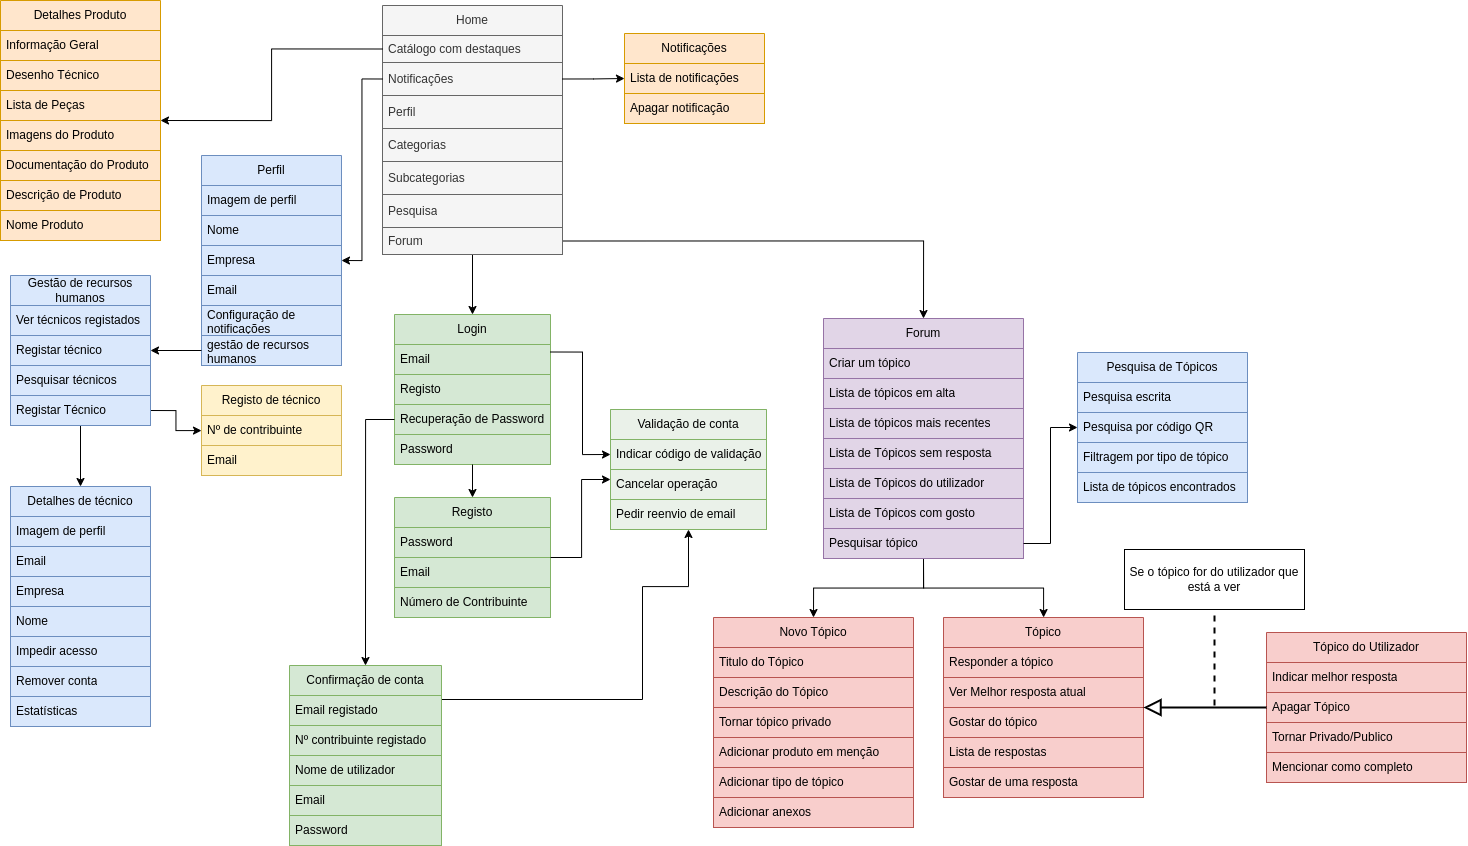
\includegraphics[width=\textwidth]{images/Arquiteturas/diagrama_superficial_de_aplicacao.png}
    \caption{Esquema de organização de páginas do \textit{software}}
    \label{fig:3}
\end{figure}

\newpage

\subsection{Autenticação e página Inicial}

Através deste esquema é possível perceber que do ecrã principal, o utilizador tem acesso ao 
catálogo de produtos e ao fórum, neste pode também realizar o \textit{login} e o \textit{logout} que redirecionam para os respetivos ecrãs.

No ecrã de \textit{login} é necessário o utilizador indicar o número de contribuinte e a \textit{\textit{password}}, neste ele pode também pedir recuperação de \textit{\textit{password}} e/ou redirecionar para o registo onde necessitará de número de contribuinte, \textit{\textit{password}} e \textit{email} para o realizar.

Em caso de o utilizador não possuir a conta ativa, este será encaminhado para o ecrã de validação conta em que deverá indicar o código de validação, cancelar a operação e pedir o reenvio do código de validação.

Em caso de se tratar de um técnico que necessita de confirmar a sua conta, este conseguirá ver as informações registadas, introduzir o seu nome, alterar o seu \textit{email} e \textit{password}.

\begin{figure}[htb]
    \centering
    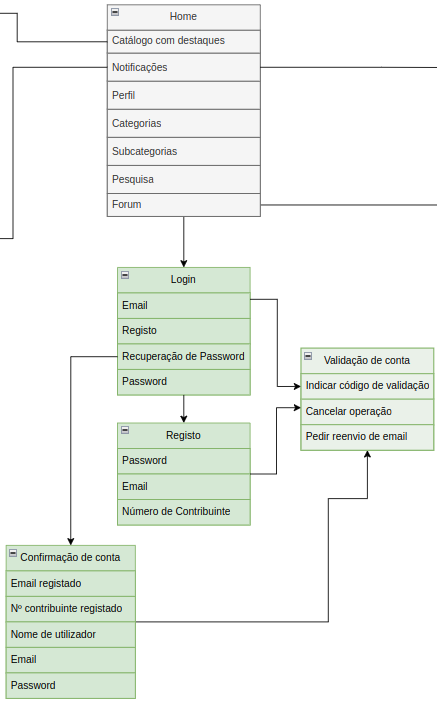
\includegraphics[height=0.9\textwidth]{images/Arquiteturas/superficial_de_app/home_auth.png}
    \caption{Esquema de organização das páginas de autenticação e página inicial}
    \label{fig:4}
\end{figure}

\newpage

\subsection{Fórum}

Através do ecrã inicial o utilizador pode direcionar-se para o ecrã do fórum. Neste ecrã, poderá pesquisar por publicações, ou então aceder a publicações em alta, mais recentes ou sem resposta.
O técnico consegue também criar e ver as suas publicações.

\begin{figure}[htb]
    \centering
    
    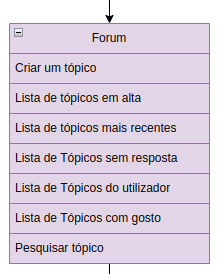
\includegraphics[height=0.4\textwidth]{images/Arquiteturas/superficial_de_app/forum.png}
    \caption{Esquema de organização da página de fórum}
    \label{fig:5}
\end{figure}

\subsection{Criar nova publicação}

Quando o técnico decide criar uma publicação, este tem de indicar o título e a descrição, de seguida poderá indicar se é privado ou não, o tipo de publicação, o produto referente e adicionar anexos.

\begin{figure}[htb]
    \centering
    
    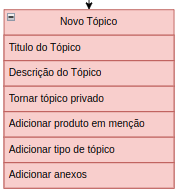
\includegraphics[height=0.3\textwidth]{images/Arquiteturas/superficial_de_app/criar_topico.png}
    \caption{Esquema de organização da página de criação de publicações}
    \label{fig:6}
\end{figure}

\newpage

\subsection{Detalhes de publicações}

O técnico pode também ver os detalhes da publicação, responder, 
gostar e gostar de uma resposta.
Caso esta seja do mesmo, este pode indicar a melhor resposta, apagar a publicação, tornar pública ou privada e indicar como completa.

\begin{figure}[htb]
    \centering
    
    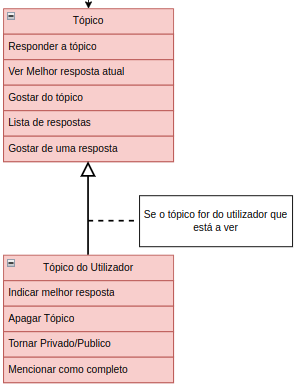
\includegraphics[height=0.55\textwidth]{images/Arquiteturas/superficial_de_app/detalhes_topico.png}
    \caption{Esquema de organização da página de detalhes de publicação}
    \label{fig:7}
\end{figure}

\subsection{Pesquisa de tópicos}

A página de pesquisa permite ao técnico procurar por tópicos específicos tanto por nome como por produto. Para além da pesquisa o utilizador pode também realizar a filtragem dos 
tópicos por tipo e categoria.
\begin{figure}[htb]
    \centering
    
    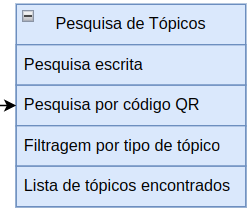
\includegraphics[height=0.3\textwidth]{images/Arquiteturas/superficial_de_app/pesquisa_forum.png}
    \caption{Esquema de organização da página de pesquisa de tópicos}
    \label{fig:8}
\end{figure}

\subsection{Notificações}

A página de notificações permite ao técnico visualizar as suas notificações, assim como também apagar.
\begin{figure}[htb]
    \centering
    
    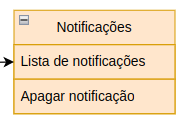
\includegraphics[height=0.2\textwidth]{images/Arquiteturas/superficial_de_app/notificacoes.png}
    \caption{Esquema de organização da página de notificações}
    \label{fig:9}
\end{figure}

\subsection{Perfil}

A página de perfil de técnico permite visualizar as suas informações, assim como alterar 
o seu \textit{email} e configurar as notificações. Caso se trate de uma empresa a visualizar o seu perfil, esta poderá ter acesso à gestão de recursos humanos, para gerir os seus técnicos.
\begin{figure}[htb]
    \centering
    
    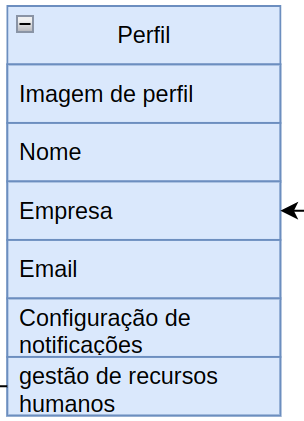
\includegraphics[height=0.35\textwidth]{images/Arquiteturas/superficial_de_app/perfil.png}
    \caption{Esquema de organização da página de notificações}
    \label{fig:10}
\end{figure}

\newpage

\subsection{Gestão de recursos humanos}

A página de gestão de recursos humanos permite à empresa gerir todos os seus técnicos registados e criar contas. Assim que a empresa seleciona um técnico, esta vê o seu perfil, 
com estatísticas.
\begin{figure}[htb]
    \centering
    
    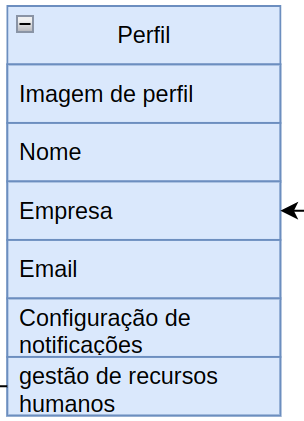
\includegraphics[height=0.35\textwidth]{images/Arquiteturas/superficial_de_app/perfil.png}
    \caption{Esquema de organização da página de gestão de recursos humanos}
    \label{fig:11}
\end{figure}